\makeatletter
\@ifundefined{keepfig}{\newenvironment{keepfig}{\par\edef\keepfig@pi{\the\parindent}\noindent
  \begin{minipage}{\linewidth}\parindent=\keepfig@pi\relax}{\end{minipage}\par}}{}
\makeatother
\section{Построения циркулем и линейкой}

Греки хорошо понимали целые и рациональные числа и были поражены, обнаружив, что длина диагонали квадрата со
стороной $1$, т.\,е.\ $\sqrt2$, не рациональна. Так они поняли, что систему чисел нужно расширять, и надеялись, что
достаточно будет чисел, которые можно <<построить>> циркулем и линейкой. Это привело к трём знаменитым задачам,
которые они так и не решили: можно ли циркулем и линейкой \emph{удвоить куб}, \emph{разделить угол на три равные
части} (трисекция угла) и \emph{построить квадрат, равновеликий данному кругу} (квадратура круга)? Мы увидим, что ответ во
всех трёх случаях отрицателен, причём доказательство целиком алгебраическое: построения переводятся на язык
расширений полей, и всё решают степени расширений.

\subsection*{Постановка задачи}

На плоскости $\R\times\R$ даны две точки $O=(0,0)$ и $I=(1,0)$; расстояние между ними~--- единица длины. Разрешается
выполнять следующие действия:
\begin{itemize}
\item провести прямую (линейкой) через две уже построенные точки;
\item провести окружность (циркулем) с центром в уже построенной точке и радиусом, равным расстоянию между двумя уже
построенными точками;
\item отметить точки пересечения уже проведённых прямых и окружностей.
\end{itemize}
Точка \emph{построима}, если её можно получить конечной последовательностью таких действий. Вещественное число $\alpha$
называется \emph{построимым}, если построима точка $(\alpha,0)$; равносильно, если отрезок длины $|\alpha|$ можно
построить (отложив его от точки $O$ по оси $OI$). Ниже (в доказательстве \rf{1.36}) мы увидим, что точка $(a,b)$
построима тогда и только тогда, когда построимы обе её координаты.

\begin{aside}[1.34c: зачем нужен единичный отрезок]
Может показаться, что единица лишняя: например, по отрезкам длины $c$ и $d$ хочется построить отрезок длины $cd$. Но без
единицы это невозможно, и дело не в технике, а в постановке: длина $cd$ зависит от выбора единицы измерения. Строго:
пусть некоторая процедура по любым отрезкам длины $c$ и $d$ строит отрезок длины $cd$. Применим ко всему чертежу
гомотетию с коэффициентом $\lambda\ne1$, $\lambda>0$. Прямые переходят в прямые, окружности~--- в окружности, пересечения~---
в пересечения, поэтому получится правильное выполнение той же процедуры для отрезков $\lambda c$ и $\lambda d$, и её
результатом будет отрезок длины $\lambda cd$, а не $(\lambda c)(\lambda d)=\lambda^2cd$. Противоречие (при $cd\ne0$). Без единицы
строятся только величины, однородные первой степени относительно масштаба: $c\pm d$, $\frac{cd}e$ (по трём отрезкам),
$\sqrt{cd}$. Поэтому в задачах на построение единичный отрезок всегда считается данным.
\end{aside}

Пусть $F$~--- подполе $\R$. Для положительного $a\in F$ через $\sqrt a$ обозначается положительный квадратный корень из $a$
в $\R$. \emph{$F$-плоскость}~--- это $F\times F\subset\R\times\R$. Назовём \emph{$F$-прямой} прямую, проходящую через две точки
$F$-плоскости; это в точности прямые, заданные уравнениями
\[
ax+by+c=0,\qquad a,b,c\in F,\ (a,b)\ne(0,0).
\]
Назовём \emph{$F$-окружностью} окружность, заданную уравнением
\[
(x-a)^2+(y-b)^2=c,\qquad a,b,c\in F,\ c>0,
\]
т.\,е.\ окружность с центром в $F$-точке, квадрат радиуса которой лежит в $F$. Например, окружность с центром в
$F$-точке и радиусом, равным расстоянию между двумя $F$-точками $(x_1,y_1)$ и $(x_2,y_2)$, есть $F$-окружность:
квадрат радиуса $(x_1-x_2)^2+(y_1-y_2)^2$ лежит в $F$ (сам радиус, вообще говоря, в $F$ не лежит).

\begin{lemma}[1.35]
Пусть $L\ne L'$~--- $F$-прямые, $C\ne C'$~--- $F$-окружности.
\begin{enumerate}[label=(\alph*)]
\item $L\cap L'$ либо пусто, либо состоит из одной $F$-точки.
\item $L\cap C$ либо пусто, либо состоит из одной или двух точек $F[\sqrt e]$-плоскости для некоторого $e\in F$, $e>0$.
\item $C\cap C'$ либо пусто, либо состоит из одной или двух точек $F[\sqrt e]$-плоскости для некоторого $e\in F$, $e>0$.
\end{enumerate}
\end{lemma}

\begin{proof}
Точки пересечения находятся решением системы уравнений; покажем, что в худшем случае приходится решать квадратное
уравнение с коэффициентами из $F$.

(a) Система $ax+by+c=0$, $a'x+b'y+c'=0$ с коэффициентами из $F$ либо не имеет решений (параллельные прямые), либо
при $ab'-a'b\ne0$ имеет единственное решение, которое по правилу Крамера выражается через коэффициенты
арифметическими операциями и потому лежит в $F\times F$. (Случай бесконечного числа решений означает $L=L'$.)

(b) Пусть $L\colon ax+by+c=0$, $C\colon(x-u)^2+(y-v)^2=w$ ($u,v,w\in F$) и, скажем, $b\ne0$ (иначе поменяем ролями $x$ и
$y$). Тогда $y=-(ax+c)/b$; подставив это в уравнение $C$, получим уравнение $Ax^2+Bx+D=0$ с $A,B,D\in F$, $A=1+a^2/b^2\ne0$. Если его дискриминант
$e=B^2-4AD$ отрицателен, пересечение пусто; иначе $x=\frac{-B\pm\sqrt e}{2A}\in F[\sqrt e]$ и $y=-(ax+c)/b\in F[\sqrt e]$.
(При $e=0$ точка одна, и она даже лежит в $F$-плоскости; в этом случае можно взять, например, $e=1$.)

(c) Вычтем уравнения окружностей $x^2+y^2-2ax-2by+(a^2+b^2-c)=0$ и $x^2+y^2-2a'x-2b'y+(a'^2+b'^2-c')=0$:
квадратичные члены сокращаются, и получается уравнение
\[
2(a'-a)x+2(b'-b)y+(a^2+b^2-c)-(a'^2+b'^2-c')=0 .
\]
Если $(a,b)=(a',b')$, то окружности концентрические и различны, т.\,е.\ $c\ne c'$, и пересечение пусто. Иначе это
уравнение $F$-прямой $L$, и $C\cap C'=C\cap L$; остаётся применить (b).
\end{proof}

\subsection*{Элементарные построения}

Сначала напомним школьные построения, на которых всё держится.

\begin{lemma}[1.35a]
Циркулем и линейкой можно:
\begin{enumerate}[label=(\alph*)]
\item провести перпендикуляр к данной прямой $l$ через данную точку $P$ (лежащую на $l$ или нет);
\item провести прямую, параллельную $l$, через данную точку $P\notin l$;
\item отложить на данной прямой от данной точки отрезок данной длины;
\item отложить от данного луча угол, равный данному.
\end{enumerate}
\end{lemma}

\begin{proof}
(a) Пусть $P\in l$. Окружность с центром $P$ произвольного (построимого) радиуса пересекает $l$ в точках $A$ и $B$, и
$P$~--- середина $AB$. Окружности радиуса $AB$ с центрами $A$ и $B$ пересекаются в точках $Q$, $Q'$, для которых
треугольники $ABQ$ и $ABQ'$ равносторонние. Прямая $QQ'$~--- серединный перпендикуляр к $AB$ (каждая точка $Q,Q'$
равноудалена от $A$ и $B$); она проходит через $P$ и перпендикулярна $l$. (Иначе: $QP$~--- медиана равностороннего
треугольника $ABQ$, а значит, и его высота.)

Пусть $P\notin l$. Окружность с центром $P$ достаточно большого радиуса пересекает $l$ в двух точках $A$, $B$. Окружности с
центрами $A$ и $B$ радиуса $AP=BP$ пересекаются в $P$ и ещё в одной точке $P'$. Четырёхугольник $APBP'$~--- ромб (все
стороны равны $AP$), а диагонали ромба перпендикулярны; значит, $PP'\perp AB=l$.

(b) Опустим из $P$ перпендикуляр $m$ на $l$ и проведём через $P$ перпендикуляр к $m$; он параллелен $l$.

(c) Окружность с центром в данной точке и радиусом, равным данному отрезку, пересекает прямую в двух точках.

(d) Пусть дан угол с вершиной $A$ и луч с началом $A'$. Окружность произвольного (построимого) радиуса $r$ с центром $A$
пересекает стороны угла в точках $X$ и $Y$, окружность того же радиуса с центром $A'$ пересекает луч в точке $X'$, а
окружность радиуса $XY\le2r$ с центром $X'$ пересекает её в точке $Y'$ (в любой из двух полуплоскостей). Треугольники
$AXY$ и $A'X'Y'$ равны по трём сторонам, поэтому $\angle X'A'Y'=\angle XAY$.
\end{proof}

\begin{center}
\begin{keepfig}
\centering
\begin{tikzpicture}[scale=0.95,every node/.style={font=\small}]
% перпендикуляр в точке прямой
\begin{scope}
\draw[cold,thick] (-2.6,0) -- (2.6,0) node[right] {$l$};
\fill[cold] (0,0) circle (1.6pt) node[below right=-1pt] {$P$};
\draw[gray] (0,0) circle (1);
\fill (-1,0) circle (1.4pt) node[below left=-1pt] {$A$};
\fill (1,0) circle (1.4pt) node[below right=-1pt] {$B$};
\draw[gray!70,dashed] (-1,0) circle (2);
\draw[gray!70,dashed] (1,0) circle (2);
\fill[cnew] (0,1.732) circle (1.5pt) node[above left=-1pt] {$Q$};
\fill[cnew] (0,-1.732) circle (1.5pt) node[below left=-1pt] {$Q'$};
\draw[cnew,thick] (0,-2.3) -- (0,2.3);
\draw[cnew!70] (-1,0) -- (0,1.732) -- (1,0);
\end{scope}
% перпендикуляр из точки вне прямой
\begin{scope}[xshift=6.6cm]
\draw[cold,thick] (-2.6,0) -- (2.6,0) node[right] {$l$};
\fill[cold] (0.3,1.2) circle (1.6pt) node[above right=-1pt] {$P$};
\draw[gray] (0.3,1.2) circle (1.7);
% A,B: (0.3 +- sqrt(1.7^2-1.2^2),0) = 0.3 +- 1.2042
\fill (-0.904,0) circle (1.4pt) node[below left=-1pt] {$A$};
\fill (1.504,0) circle (1.4pt) node[below right=-1pt] {$B$};
\draw[gray!70,dashed] (-0.904,0) circle (1.7);
\draw[gray!70,dashed] (1.504,0) circle (1.7);
\fill[cnew] (0.3,-1.2) circle (1.5pt) node[below right=-1pt] {$P'$};
\draw[cnew!70] (0.3,1.2) -- (-0.904,0) -- (0.3,-1.2) -- (1.504,0) -- cycle;
\draw[cnew,thick] (0.3,-2.2) -- (0.3,2.4) node[above] {$m$};
\draw[cnew,thick,dashed] (-2.6,1.2) -- (2.6,1.2) node[right] {$n\parallel l$};
\end{scope}
\end{tikzpicture}
\figcap{Перпендикуляр к прямой $l$ через точку $P$. Слева $P\in l$: прямая $QQ'$~--- серединный перпендикуляр к $AB$.
Справа $P\notin l$: $APBP'$~--- ромб, и его диагональ $m=PP'$ перпендикулярна диагонали $AB$; прямая $n$,
перпендикулярная $m$ в точке $P$, параллельна $l$ (\rf{1.35a}(b)).}
\end{keepfig}
\end{center}

\begin{center}
\begin{keepfig}
\centering
\begin{tikzpicture}[scale=1.25,every node/.style={font=\small}]
% данный угол alpha=40, r=1.2, XY=0.8208
\begin{scope}
\draw[cold,thick] (0,0) -- (2.1,0);
\draw[cold,thick] (0,0) -- (40:2.1);
\draw[gray] (1.2,0) arc (0:58:1.2);
\draw[gray!70,dashed] (1.2,0) -- (40:1.2);
\draw[cold] (0.4,0) arc (0:40:0.4); \node[cold] at (20:0.58) {$\alpha$};
\fill[cold] (0,0) circle (1.2pt) node[below left=-1pt] {$A$};
\fill (1.2,0) circle (1.2pt) node[below] {$X$};
\fill (40:1.2) circle (1.2pt) node[above left=-1pt] {$Y$};
\end{scope}
% перенос на луч с началом A'
\begin{scope}[xshift=3.2cm]
\draw[cold,thick] (0,0) -- (2.1,0);
\draw[gray] (1.2,0) arc (0:58:1.2);
\draw[gray] ($(1.2,0)+(95:0.8208)$) arc (95:125:0.8208);
\draw[cnew,thick] (0,0) -- (40:2.1);
\draw[cnew] (0.4,0) arc (0:40:0.4); \node[cnew] at (20:0.58) {$\alpha$};
\fill[cold] (0,0) circle (1.2pt) node[below left=-1pt] {$A'$};
\fill (1.2,0) circle (1.2pt) node[below] {$X'$};
\fill[cnew] (40:1.2) circle (1.3pt) node[above=2pt] {$Y'$};
\end{scope}
% удвоение: перенос на луч AY
\begin{scope}[xshift=6.6cm]
\draw[cold,thick] (0,0) -- (2.1,0);
\draw[cold,thick] (0,0) -- (40:2.1);
\draw[gray] (1.2,0) arc (0:95:1.2);
\draw[gray!70,dashed] (1.2,0) -- (40:1.2);
\draw[gray] ($(40:1.2)+(135:0.8208)$) arc (135:165:0.8208);
\draw[cnew,thick] (0,0) -- (80:2.0);
\draw[cnew] (0.45,0) arc (0:80:0.45); \node[cnew] at (60:0.72) {$2\alpha$};
\fill[cold] (0,0) circle (1.2pt) node[below left=-1pt] {$A$};
\fill (1.2,0) circle (1.2pt) node[below] {$X$};
\fill (40:1.2) circle (1.2pt) node[right=1pt] {$Y$};
\fill[cnew] (80:1.2) circle (1.3pt) node[left=1pt] {$Z$};
\end{scope}
\end{tikzpicture}
\figcap{Перенос угла (\rf{1.35a}(d)): дуги одного радиуса с центрами $A$ и $A'$, затем засечка радиуса $XY$ с
центром $X'$; треугольники $AXY$ и $A'X'Y'$ равны по трём сторонам. Справа~--- удвоение угла: тот же перенос на луч
$AY$ (засечка радиуса $XY$ с центром $Y$) даёт точку $Z$ с $\angle XAZ=2\alpha$.}
\end{keepfig}
\end{center}

Из (c) и (d) следует, что можно построить треугольник, подобный данному, на отрезке данной длины: на концах отрезка
откладываем от него два угла треугольника, а третий угол получится сам, так как сумма углов треугольника равна $\pi$.
(Можно и по теореме Фалеса: отложить данную длину на прямой, содержащей сторону треугольника, и провести параллельную
прямую, (b).) Откладывая угол от стороны другого угла, мы складываем углы (а откладывая в другую сторону~---
вычитаем); в частности, любой построенный угол можно удвоить. Именно так, через подобие, строятся произведение и
частное.

\begin{lemma}[1.36]
\begin{enumerate}[label=(\alph*)]
\item Если $c$ и $d$ построимы, то построимы и $c+d$, $-c$, $cd$ и $\frac cd$ (при $d\ne0$).
\item Если $c>0$ построимо, то построимо и $\sqrt c$.
\end{enumerate}
\end{lemma}

\begin{proof}
\emph{Оси и координаты.} Прямая $OI$~--- ось $x$; перпендикуляр к ней в точке $O$~--- ось $y$. Если точка $P=(a,b)$
построена, то основания перпендикуляров из $P$ на оси дают точки $(a,0)$ и $(0,b)$, а окружность с центром $O$ через
$(0,b)$ пересекает ось $x$ в точках $(\pm b,0)$. Обратно, по точкам $(a,0)$ и $(b,0)$ строятся $(0,b)$ (окружность с
центром $O$) и затем $(a,b)$~--- пересечение перпендикуляров к осям в точках $(a,0)$ и $(0,b)$. Итак, точка построима
тогда и только тогда, когда построимы обе её координаты.

(a) Окружность с центром $O$ через $(c,0)$ пересекает ось $x$ ещё в точке $(-c,0)$. Окружность с центром $(c,0)$ и
радиусом $|d|$ (расстояние от $O$ до $(d,0)$) пересекает ось $x$ в точках $(c\pm|d|,0)$, среди которых есть $c+d$. Для
произведения и частного достаточно (с учётом $-c$) рассмотреть $c,d>0$. Отметим точки $A=(1,0)$, $A'=(d,0)$ на оси
$x$ и $B=(0,c)$ на оси $y$, проведём прямую $AB$ и параллельную ей прямую через $A'$; она пересечёт ось $y$ в точке
$B'$. Треугольники $OAB$ и $OA'B'$ подобны (теорема Фалеса), поэтому $OB'/OB=OA'/OA$, т.\,е.\ $OB'=cd$. (Положение $d$
относительно $1$ роли не играет: при $d<1$ точка $A'$ лежит между $O$ и $A$, а $B'$~--- между $O$ и $B$.) Если же взять
$A=(d,0)$, $A'=(1,0)$, то тем же построением получим $OB'=c\cdot\frac1d=\frac cd$.

(b) Проведём окружность с центром $\bigl(\frac{c+1}2,0\bigr)$ и радиусом $\frac{c+1}2$ (оба числа построимы по (a)); она
проходит через $O$ и через $(c+1,0)$, т.\,е.\ это окружность с диаметром длины $1+c$, разбитым точкой $A=(1,0)$ на
отрезки $1$ и $c$. Перпендикуляр к оси $x$ в точке $A$ пересекает окружность в точке $P=(1,y)$, $y>0$, и
\[
y^2=\Bigl(\frac{c+1}2\Bigr)^2-\Bigl(1-\frac{c+1}2\Bigr)^2=\Bigl(\frac{c+1}2\Bigr)^2-\Bigl(\frac{c-1}2\Bigr)^2=c,
\]
т.\,е.\ $AP=\sqrt c$. (При $c>1$ центр окружности лежит правее $A$, при $c<1$~--- левее; вычисление от этого не
зависит.) Геометрически: высота прямоугольного треугольника, опущенная на гипотенузу, есть среднее
геометрическое отрезков, на которые она делит гипотенузу (треугольник с вершиной $P$, опирающийся на диаметр,
прямоугольный).
\end{proof}

\begin{center}
\begin{keepfig}
\centering
\begin{tikzpicture}[scale=0.95,every node/.style={font=\small},>=stealth]
% произведение по Фалесу: c=1.3, d=2.2
\begin{scope}
\draw[->,gray] (-0.3,0) -- (3.0,0) node[right] {$x$};
\draw[->,gray] (0,-0.3) -- (0,3.3) node[above] {$y$};
\fill (0,0) circle (1.4pt) node[below left] {$O$};
\fill[cold] (1,0) circle (1.6pt) node[below] {$A{=}1$};
\fill[cold] (2.2,0) circle (1.6pt) node[below] {$A'{=}d$};
\fill[cold] (0,1.3) circle (1.6pt) node[left] {$B{=}c$};
\draw[cold,thick] (1,0) -- (0,1.3);
\draw[cnew,thick] (2.2,0) -- (0,2.86);
\fill[cnew] (0,2.86) circle (1.6pt) node[left] {$B'{=}cd$};
\end{scope}
% квадратный корень: c=2.5
\begin{scope}[xshift=5.2cm]
\draw[->,gray] (-0.3,0) -- (3.9,0) node[right] {$x$};
\draw[gray] (1.75,0) circle (1.75);
\fill (0,0) circle (1.4pt) node[above left] {$O$};
\fill[cold] (1,0) circle (1.6pt) node[below left=-1pt] {$A$};
\fill (1.75,0) circle (1.3pt) node[below right=-1pt] {$M$};
\fill (3.5,0) circle (1.4pt);
\draw[cnew,thick] (1,-0.3) -- (1,2.0);
\fill[cnew] (1,1.581) circle (1.6pt) node[above left] {$P$};
\draw[cnew!60] (0,0) -- (1,1.581) -- (3.5,0);
\draw[cnew!60] (1.75,0) -- (1,1.581);
\draw[decorate,decoration={brace,mirror,amplitude=3pt}] (0.1,-0.45) -- (0.98,-0.45) node[midway,below=2pt] {$1$};
\draw[decorate,decoration={brace,mirror,amplitude=3pt}] (1.02,-0.45) -- (3.4,-0.45) node[midway,below=2pt] {$c$};
\node[cnew,right] at (1,0.75) {$\sqrt c$};
\end{scope}
\end{tikzpicture}
\figcap{Слева: произведение. Прямая через $A'$ параллельна $AB$, и из подобия $OAB\sim OA'B'$ получаем $OB'=cd$;
поменяв местами $1$ и $d$ на оси $x$, получим $c/d$. Справа: квадратный корень. Окружность с центром $M=\bigl(\frac{c+1}2,0\bigr)$ и диаметром $1+c$;
перпендикуляр в точке $A$, делящей диаметр на отрезки $1$ и $c$, имеет длину $AP=\sqrt c$.}
\end{keepfig}
\end{center}

\begin{remark}[1.36a: катет~--- среднее геометрическое]
В прямоугольном треугольнике $ABC$ с прямым углом $B$ и высотой $BH$ треугольники $ABH$ и $ACB$ подобны (общий острый
угол $A$), поэтому $\frac{AB}{AC}=\frac{AH}{AB}$, т.\,е.\ $AB^2=AC\cdot AH$: катет есть среднее геометрическое гипотенузы и
своей проекции на неё. Это даёт ещё одно построение чисел $\frac1c$ и $\sqrt c$ при $c>0$, $c\ne1$.
\begin{itemize}[leftmargin=*]
\item $\frac1c$. Если $c>1$, построим прямоугольный треугольник с катетом $AB=1$ и гипотенузой $AC=c$ (перпендикуляр к
$AB$ в точке $B$ пересекает окружность радиуса $c$ с центром $A$, так как $c>1$) и опустим высоту $BH$; тогда
$AH=\frac1c$. Если $c<1$, отложим $AH=c$, отметим на перпендикуляре к $AH$ в точке $H$ точку $B$ с $AB=1$ (она есть,
так как $c<1$) и проведём через $B$ перпендикуляр к $AB$; он пересечёт прямую $AH$ в точке $C$, и $AC=\frac1c$.
\item $\sqrt c$. Отметим на прямой точки $A$, $H$, $C$ ($H$ между $A$ и $C$) с $AH=1$, $AC=c$ при $c>1$ (соответственно
$AH=c$, $AC=1$ при $c<1$), и пусть $B$~--- точка пересечения перпендикуляра к $AC$ в точке $H$ с окружностью на
диаметре $AC$ (угол $ABC$, опирающийся на диаметр, прямой). Тогда $AB=\sqrt{AC\cdot AH}=\sqrt c$.
\end{itemize}
\end{remark}

\begin{center}
\begin{keepfig}
\centering
\begin{tikzpicture}[scale=1.5,every node/.style={font=\small}]
% c=3: A=(0,0), C=(3,0), B=(1/3, sqrt(8)/3), H=(1/3,0)
\coordinate (A) at (0,0); \coordinate (C) at (3,0); \coordinate (B) at ({1/3},{sqrt(8)/3}); \coordinate (H) at ({1/3},0);
\draw[gray] (3,0) arc (0:180:1.5);
\draw[thick] (B) -- (C);
\draw[cold,thick] (A) -- (C);
\draw[cold,thick] (A) -- (B);
\draw[cnew,thick] (B) -- (H);
\draw[cnew] ($(H)+(0,0.12)$) -- ++(0.12,0) -- ++(0,-0.12);
\draw ($(B)!0.14cm!(A)$) -- ($(B)!0.14cm!(A)+(B)!0.14cm!(C)-(B)$) -- ($(B)!0.14cm!(C)$);
\fill (A) circle (1.2pt) node[below left=-1pt] {$A$};
\fill (B) circle (1.2pt) node[above] {$B$};
\fill (C) circle (1.2pt) node[below right=-1pt] {$C$};
\fill[cnew] (H) circle (1.2pt) node[below right=-1pt] {$H$};
\draw[decorate,decoration={brace,mirror,amplitude=3pt}] (0.02,-0.3) -- (0.32,-0.3) node[midway,below=2pt,cnew] {$\frac1c$};
\draw[decorate,decoration={brace,mirror,amplitude=4pt}] (0,-0.75) -- (3,-0.75) node[midway,below=3pt,cold] {$c$};
\node[cold,left] at (0.15,0.5) {$1$};
\end{tikzpicture}
\figcap{Катет~--- среднее геометрическое гипотенузы и своей проекции на неё: $AB^2=AC\cdot AH$. При $AB=1$, $AC=c$
получаем $AH=\frac1c$ (здесь $c=3$); при $AH=1$, $AC=c$ получаем $AB=\sqrt c$.}
\end{keepfig}
\end{center}

\begin{theorem}[1.37]
\begin{enumerate}[label=(\alph*)]
\item Построимые числа образуют подполе $\R$.
\item Число $\alpha$ построимо тогда и только тогда, когда оно лежит в подполе $\R$ вида
\[
\Q[\sqrt{a_1},\dots,\sqrt{a_r}],\qquad a_i\in\Q[\sqrt{a_1},\dots,\sqrt{a_{i-1}}],\quad a_i>0 .
\]
\end{enumerate}
\end{theorem}

\begin{proof}
(a) Это переформулировка \rf{1.36}(a) ($0$ и $1$ построимы по определению).

(b) Пусть точки $P_1,\dots,P_n$ получены последовательно: $P_1=O$, $P_2=I$, а каждая следующая~--- точка пересечения
прямых и окружностей, проведённых по предыдущим точкам. Докажем индукцией по $k$, что все координаты точек
$P_1,\dots,P_k$ лежат в некотором поле $K_k$ вида, указанного в (b). Для $k=2$ годится $K_2=\Q$. Пусть утверждение верно
для $k-1$. Прямая через две $K_{k-1}$-точки~--- $K_{k-1}$-прямая, окружность с центром в $K_{k-1}$-точке и радиусом,
равным расстоянию между $K_{k-1}$-точками,~--- $K_{k-1}$-окружность. По лемме \rf{1.35} координаты $P_k$ лежат в
$K_{k-1}[\sqrt e]$ с $e\in K_{k-1}$, $e>0$; положим $K_k=K_{k-1}[\sqrt e]$. Значит, каждое построимое число (абсцисса
построимой точки) лежит в поле вида $\Q[\sqrt{a_1},\dots,\sqrt{a_r}]$.

Обратно, пусть все элементы $\Q[\sqrt{a_1},\dots,\sqrt{a_{i-1}}]$ построимы. Тогда $a_i$ построимо, и по \rf{1.36}(b) построимо
$\sqrt{a_i}$; по (a) построимы все элементы $\Q[\sqrt{a_1},\dots,\sqrt{a_i}]$ (это многочлены от $\sqrt{a_i}$ с коэффициентами
из предыдущего поля). Применяя это при $i=1,2,\dots,r$, получаем, что все элементы $\Q[\sqrt{a_1},\dots,\sqrt{a_r}]$
построимы.
\end{proof}

\begin{corollary}[1.38]
Если $\alpha$ построимо, то $\alpha$ алгебраично над $\Q$ и $[\Q[\alpha]:\Q]$~--- степень двойки.
\end{corollary}

\begin{proof}
Пусть $\alpha\in K_r=\Q[\sqrt{a_1},\dots,\sqrt{a_r}]$, $K_i=\Q[\sqrt{a_1},\dots,\sqrt{a_i}]$. На каждом шаге
$K_i=K_{i-1}[\sqrt{a_i}]$ присоединяется корень многочлена $X^2-a_i\in K_{i-1}[X]$, поэтому $[K_i:K_{i-1}]$ равно $1$ (если
$\sqrt{a_i}\in K_{i-1}$) или $2$. По мультипликативности степеней \rf{1.20} $[K_r:\Q]=2^s$ для некоторого $s$; в частности,
$K_r$ конечно над $\Q$, и $\alpha$ алгебраично (\rf{1.30}). Наконец, $\Q\subset\Q[\alpha]\subset K_r$, и по \rf{1.20} степень
$[\Q[\alpha]:\Q]$ делит $[K_r:\Q]$, поэтому тоже является степенью двойки.
\end{proof}

\begin{center}
\begin{keepfig}
\centering
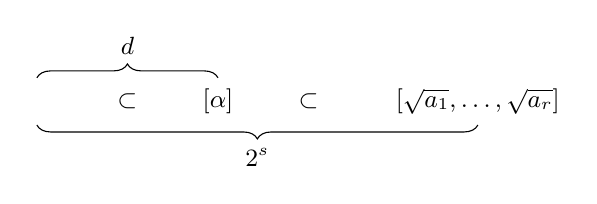
\begin{tikzpicture}[every node/.style={font=\small}]
\node (Q) at (0,0) {$\Q$};
\node (A) at (2.3,0) {$\Q[\alpha]$};
\node (K) at (5.6,0) {$\Q[\sqrt{a_1},\dots,\sqrt{a_r}]$};
\node at (1.15,0) {$\subset$};
\node at (3.45,0) {$\subset$};
\draw[decorate,decoration={brace,amplitude=5pt}] (0,0.3) -- (2.3,0.3) node[midway,above=5pt] {$d$};
\draw[decorate,decoration={brace,mirror,amplitude=5pt}] (0,-0.3) -- (5.6,-0.3) node[midway,below=5pt] {$2^s$};
\end{tikzpicture}
\figcap{Степень $d=[\Q[\alpha]:\Q]$ делит $2^s$, поэтому $d=2^t$.}
\end{keepfig}
\end{center}

\begin{remark}[1.38a: что даёт и чего не даёт \rf{1.38}]
Теорема \rf{1.37}(b)~--- точный критерий, но в терминах башен, а не в терминах самого числа $\alpha$. Следствие \rf{1.38}
даёт лишь \emph{необходимое} условие построимости: обратное к нему неверно. Например, многочлен $X^4-X-1$ неприводим
над $\Q$ (он неприводим даже по модулю $2$: у $X^4+X+1$ нет корней в $\F_2$, и он не делится на $X^2+X+1$~---
единственный неприводимый многочлен степени $2$ над $\F_2$, так как $(X^2+X+1)^2=X^4+X^2+1$; см.\ \rf{1.18} и \rf{1.18a}(b)),
так что его вещественные корни имеют степень $4$, но ни один из них не построим: группа Галуа этого многочлена~---
$S_4$, а поле его разложения имеет степень $24$ (его дискриминант $-283$ не квадрат, а кубическая резольвента
$X^3+4X-1$ (\rf{4.9}) не имеет рациональных корней и потому неприводима; отсюда, как в \rf{4.10}, группа Галуа~---
$S_4$; ср.\ пример $X^4-4X+2$ в \rf{3.27}). Точный критерий формулируется с помощью теории Галуа: вещественное число $\alpha$ построимо тогда и только
тогда, когда оно алгебраично и поле разложения $E$ его минимального многочлена над $\Q$ имеет степень $2^r$.

Действительно, если $[E:\Q]=2^r$, то $G=\Gal(E/\Q)$~--- $2$-группа, и между её подгруппой $H=\Gal(E/\Q[\alpha])$ и $G$ есть
цепочка подгрупп с индексами $2$ (свойство конечных $p$-групп). По основной теореме теории Галуа (\rf{3.17}) ей
отвечает цепочка полей $\Q=L_0\subset L_1\subset\dots\subset L_m=\Q[\alpha]\subset\R$ со ступенями степени $2$, а каждое
квадратичное расширение имеет вид $L_{i}=L_{i-1}[\sqrt{d_i}]$ (\rf{3.25}), причём $d_i>0$, так как $L_i\subset\R$; по \rf{1.37}(b)
число $\alpha$ построимо. Так же (с цепочкой от $\{1\}$ до $G$ в вещественном поле Галуа) доказывается теорема \rf{3.24}. Обратно, если $\alpha\in\Q[\sqrt{a_1},\dots,\sqrt{a_r}]$,
то поле, порождённое образами этой башни при всех вложениях в $\CC$, снова получается последовательным
присоединением квадратных корней, имеет степень $2^s$ над $\Q$ и содержит все корни минимального многочлена $\alpha$;
поэтому $[E:\Q]$ делит $2^s$. Для трёх классических задач хватает и одностороннего утверждения \rf{1.38}.
\end{remark}

\subsection*{Три классические задачи}

\begin{corollary}[1.39]
Удвоить куб циркулем и линейкой невозможно.
\end{corollary}

\begin{proof}
Задача состоит в том, чтобы по ребру $1$ построить ребро куба объёмом $2$, т.\,е.\ построить вещественный корень
$\sqrt[3]2$ многочлена $X^3-2$. Этот многочлен неприводим над $\Q$ (критерий Эйзенштейна \rf{1.16} при $p=2$), поэтому
$[\Q[\sqrt[3]2]:\Q]=3$~--- не степень двойки, и по \rf{1.38} число $\sqrt[3]2$ не построимо.
\end{proof}

Прежде чем говорить о трисекции, уточним, что значит <<построить угол>>. Угол $\theta$ задан, если построены его вершина
и по точке на каждой из сторон; перенося угол (\rf{1.35a}(d)), можно считать, что вершина~--- $O$, а одна из
сторон~--- луч $OI$.
\emph{Знать угол~--- то же, что знать его косинус}: если угол $\theta$ построен, то окружность с центром $O$ радиуса
$1$ пересекает вторую сторону в точке $P=(\cos\theta,\sin\theta)$, и основание перпендикуляра из $P$ на ось $x$ даёт
$\cos\theta$. Обратно, если построено $\cos\theta$, то перпендикуляр к оси $x$ в точке $(\cos\theta,0)$ пересекает
единичную окружность в точке $P$, и угол $IOP$ равен $\theta$ (при $0<\theta<\pi$).

\begin{center}
\begin{keepfig}
\centering
\begin{tikzpicture}[scale=1.5,every node/.style={font=\small}]
\draw[->,gray] (-0.3,0) -- (1.45,0) node[right] {$x$};
\draw[gray] (1,0) arc (0:100:1);
\fill (0,0) circle (1pt) node[below left] {$O$};
\fill[cold] (1,0) circle (1pt) node[below right] {$I$};
\draw[cold,thick] (0,0) -- (1.25,0);
\draw[cold,thick] (0,0) -- ({1.25*cos(55)},{1.25*sin(55)});
\node[gray,font=\footnotesize] at ({0.5*cos(55)-0.08},{0.5*sin(55)+0.06}) {$1$};
\fill[cnew] ({cos(55)},{sin(55)}) circle (1pt) node[right=2pt] {$P$};
\draw[cnew,thick,dashed] ({cos(55)},{sin(55)}) -- ({cos(55)},0);
\fill[cnew] ({cos(55)},0) circle (1pt);
\draw[cold] (0.25,0) arc (0:55:0.25);
\node[cold] at (0.37,0.16) {$\theta$};
\draw[decorate,decoration={brace,mirror,amplitude=3pt}] (0,-0.08) -- ({cos(55)},-0.08) node[midway,below=2pt,cnew] {$\cos\theta$};
\end{tikzpicture}
\figcap{Угол $\theta$ и его косинус строятся друг по другу: $P$~--- точка единичной окружности на стороне угла, $\cos\theta$~---
её проекция на ось $x$.}
\end{keepfig}
\end{center}

\begin{corollary}[1.40]
Произвольный угол разделить на три равные части циркулем и линейкой невозможно.
\end{corollary}

\begin{proof}
Достаточно предъявить один построимый угол, треть которого не построима. Возьмём угол $3\theta=60^\circ$: он
построим (угол равностороннего треугольника; $\cos60^\circ=\frac12$). Из формул $\cos2x=2\cos^2x-1$ и
\[
\cos3x=\cos2x\cos x-\sin2x\sin x=(2\cos^2x-1)\cos x-2\cos x(1-\cos^2x)=4\cos^3x-3\cos x
\]
следует, что $\alpha=\cos20^\circ$ удовлетворяет уравнению $4\alpha^3-3\alpha=\frac12$, т.\,е.\ является корнем многочлена
$8X^3-6X-1$. Он неприводим над $\Q$: иначе у него был бы множитель степени $1$, т.\,е.\ рациональный корень. Удобнее
положить $M=2X$: получится $M^3-3M-1$, неприводимость которого доказана в \rf{1.12} (рациональные корни унитарного
целочисленного многочлена~--- целые делители свободного члена, \rf{1.11}, т.\,е.\ $\pm1$; но $1-3-1\ne0$ и
$-1+3-1\ne0$). Значит, $[\Q[\cos20^\circ]:\Q]=3$, и по
\rf{1.38} угол $20^\circ$ не построим, хотя угол $60^\circ$ построим.
\end{proof}

Некоторые углы, конечно, делятся на три: например, $90^\circ$ (угол $30^\circ$ построим) или любой угол $3\theta$, где угол
$\theta$ построим. Утверждение \rf{1.40} говорит, что не существует построения, которое делит на три \emph{любой} угол.

\begin{corollary}[1.41]
Квадратура круга циркулем и линейкой невозможна.
\end{corollary}

\begin{proof}
Квадрат той же площади, что и круг радиуса $1$, имеет сторону $\sqrt\pi$. Число $\pi$ трансцендентно (теорема
Линдемана, 1882; доказательство мы не приводим, ср.\ раздел о трансцендентных числах), поэтому трансцендентно и
$\sqrt\pi$: если бы $\sqrt\pi$ было алгебраическим, то поле $\Q[\sqrt\pi]$ было бы конечным над $\Q$, и
$\pi=(\sqrt\pi)^2\in\Q[\sqrt\pi]$ было бы алгебраическим (\rf{1.30}). По \rf{1.38} число $\sqrt\pi$ не построимо.
\end{proof}

\subsection*{Правильные многоугольники}

Ещё одна задача, восходящая к древним грекам: при каких $n$ правильный $n$-угольник можно построить циркулем и
линейкой? Здесь мы рассмотрим простые $n=p$ (общий случай~--- теорема \rf{5.12}). Многочлен $X^p-1$ приводим:
\[
X^p-1=(X-1)(X^{p-1}+X^{p-2}+\dots+1).
\]

\begin{lemma}[1.42]
Если $p$ простое, то многочлен $X^{p-1}+\dots+X+1$ неприводим над $\Q$; следовательно, $[\Q[e^{2\pi i/p}]:\Q]=p-1$.
\end{lemma}

\begin{proof}
Пусть $f(X)=\frac{X^p-1}{X-1}=X^{p-1}+\dots+1$. Его неприводимость уже доказана в \rf{1.16a}(c): к многочлену $f(X+1)$
применяется критерий Эйзенштейна \rf{1.16} при простом $p$. Число
$\zeta=e^{2\pi i/p}\ne1$~--- корень $X^p-1$, поэтому $f(\zeta)=0$, и $f$~--- минимальный многочлен $\zeta$. Так как $\Q[\zeta]\cong\Q[X]/(f)$,
по \rf{1.25} $[\Q[\zeta]:\Q]=\deg f=p-1$.
\end{proof}

Пусть $p$~--- нечётное простое. Правильный $p$-угольник построим тогда и только тогда, когда построим его центральный
угол $\frac{2\pi}p$. Действительно, если многоугольник построен, то построен и его центр~--- точка пересечения
серединных перпендикуляров к двум сторонам,~--- а с ним и центральный угол; обратно, отложив центральный угол $p$ раз
от луча $OI$ (\rf{1.35a}(d)), получим вершины многоугольника на единичной окружности. (Можно рассуждать и через
внутренний угол: диагонали из одной вершины разбивают $p$-угольник на $p-2$ треугольника, поэтому сумма его
внутренних углов равна $\pi(p-2)$, внутренний угол равен $\pi\frac{p-2}p$, а смежный с ним угол~---
$\pi-\pi\frac{p-2}p=\frac{2\pi}p$.) Итак, $p$-угольник построим тогда и только тогда, когда построимо число
\[
\cos\frac{2\pi}p=\frac{\zeta+\zeta^{-1}}2,\qquad \zeta=e^{2\pi i/p}.
\]
Имеем $\Q[\zeta]\supset\Q[\cos\frac{2\pi}p]\supset\Q$. Степень $\Q[\zeta]$ над $\Q[\cos\frac{2\pi}p]$ равна $2$: уравнение
\[
\zeta^2-2\cos\frac{2\pi}p\cdot\zeta+1=0
\]
(разделите его на $\zeta$) показывает, что она не больше $2$, а равенство $1$ означало бы $\zeta\in\Q[\cos\frac{2\pi}p]\subset\R$,
что неверно, так как $\zeta\notin\R$. Поэтому по \rf{1.20}
\[
\Bigl[\Q\bigl[\cos\tfrac{2\pi}p\bigr]:\Q\Bigr]=\frac{p-1}2 .
\]

\begin{center}
\begin{keepfig}
\centering
\begin{tikzpicture}[scale=1.3,every node/.style={font=\small}]
\begin{scope}
\foreach \k in {0,...,6}{\coordinate (V\k) at ({90+360*\k/7}:1);}
\draw[cold,thick] (V0) \foreach \k in {1,...,6}{-- (V\k)} -- cycle;
\foreach \k in {2,...,5}{\draw[cnew] (V0) -- (V\k);}
\fill[cold] (V0) circle (1.2pt);
\end{scope}
\begin{scope}[xshift=3.2cm,yshift=-0.2cm]
\node (Q) at (0,0) {$\Q$};
\node (C) at (2.3,0) {$\Q\bigl[\cos\frac{2\pi}p\bigr]$};
\node (Z) at (4.8,0) {$\Q\bigl[e^{2\pi i/p}\bigr]$};
\node at (1.05,0) {$\subset$}; \node at (3.6,0) {$\subset$};
\draw[decorate,decoration={brace,amplitude=5pt}] (0,0.35) -- (2.3,0.35) node[midway,above=5pt,cnew] {$\frac{p-1}2$};
\draw[decorate,decoration={brace,amplitude=5pt}] (2.3,0.35) -- (4.8,0.35) node[midway,above=5pt] {$2$};
\draw[decorate,decoration={brace,mirror,amplitude=5pt}] (0,-0.35) -- (4.8,-0.35) node[midway,below=5pt,cold] {$p-1$};
\end{scope}
\end{tikzpicture}
\figcap{Слева: диагонали из одной вершины разбивают $p$-угольник ($p=7$) на $p-2$ треугольника, поэтому сумма его
углов равна $\pi(p-2)$. Справа: степени в башне $\Q\subset\Q[\cos\frac{2\pi}p]\subset\Q[e^{2\pi i/p}]$.}
\end{keepfig}
\end{center}

Если правильный $p$-угольник построим, то $\frac{p-1}2$, а значит, и $p-1$~--- степень двойки (\rf{1.38}), т.\,е.\ $p=2^k+1$.
Позже (\rf{3.26}, \rf{5.12}) мы докажем и обратное. Итак, правильный $p$-угольник ($p$ нечётное простое) построим тогда и только
тогда, когда $p=2^k+1$ для некоторого целого $k\ge1$.

Число $2^k+1$ с $k\ge1$ может быть простым, только если $k$~--- степень двойки (при $k=0$ получается простое число $2$,
но нас интересуют нечётные $p$). Действительно, иначе $k=rs$ с нечётным $s>1$, и
из тождества $Y^s+1=(Y+1)(Y^{s-1}-Y^{s-2}+\dots+1)$ при $Y=2^r$ получаем
\[
2^{rs}+1=(2^r+1)\bigl((2^r)^{s-1}-(2^r)^{s-2}+\dots+1\bigr),\qquad 1<2^r+1<2^k+1 .
\]
Значит, простые $p$, для которых правильный $p$-угольник построим,~--- это в точности простые вида $2^{2^r}+1$. Их
называют \emph{простыми числами Ферма} (Ферма предполагал, что все числа $2^{2^r}+1$ простые). При $r=0,1,2,3,4$
получаются простые числа $3,5,17,257,65537$, но Эйлер показал, что $2^{32}+1=641\cdot6700417$, и других простых чисел
Ферма не известно (ожидается, что их нет, но это не доказано).

Гаусс в 18 лет нашёл явное выражение
\[
\cos\frac{2\pi}{17}=-\frac1{16}+\frac1{16}\sqrt{17}+\frac1{16}\sqrt{34-2\sqrt{17}}
+\frac18\sqrt{17+3\sqrt{17}-\sqrt{34-2\sqrt{17}}-2\sqrt{34+2\sqrt{17}}}
\]
(обе части равны $0{,}93247222\ldots$). Все подкоренные выражения положительны ($17$, $34\mp2\sqrt{17}$ и выражение
под последним корнем, равное $11{,}295\ldots$), и каждое лежит в поле, порождённом предыдущими корнями; по
\rf{1.37}(b) отсюда сразу следует, что правильный $17$-угольник построим. Этот успех побудил Гаусса стать
математиком. Ту же величину можно записать и так:
\[
\cos\frac{2\pi}{17}=-\frac1{16}+\frac1{16}\sqrt{17}+\frac1{16}\sqrt{34-2\sqrt{17}}
+\frac18\sqrt{17+3\sqrt{17}-2\sqrt{34-2\sqrt{17}}-\sqrt{170-26\sqrt{17}}}\,.
\]
Выражения под последним корнем в обеих формулах совпадают, так как
\[
2\sqrt{34+2\sqrt{17}}=\sqrt{34-2\sqrt{17}}+\sqrt{170-26\sqrt{17}}:
\]
после возведения в квадрат это равенство сводится к $2\sqrt{(34-2\sqrt{17})(170-26\sqrt{17})}=36\sqrt{17}-68$, где обе
части положительны, а их квадраты равны $26656-4896\sqrt{17}$. Откуда берётся такая формула, видно из теории Галуа: цепочка подполей
$\Q(\zeta_{17})$ со ступенями степени $2$, порождённых гауссовыми периодами (\rf{5.11e}, \rf{5.13}).

\subsection*{Построения другими инструментами}

\begin{aside}[1.42a: построения с трисектором]
Добавим к циркулю и линейке \emph{трисектор}~--- инструмент, делящий любой построенный угол на три равные части. Что
он добавляет алгебраически? Если угол $\varphi$ построен, то построено и $b=\cos\varphi\in[-1,1]$, и трисектор даёт
$y=\cos\frac\varphi3$~--- корень многочлена $4Y^3-3Y-b$ (формула для $\cos3x$ выше). При $|b|\le1$ все три корня этого
многочлена вещественны: это
\[
\cos\frac\varphi3,\qquad \cos\frac{\varphi+2\pi}3,\qquad \cos\frac{\varphi+4\pi}3 ,
\]
и все три построимы трисектором (угол $\frac{2\pi}3$ строится циркулем и линейкой, а углы складываются переносом,
\rf{1.35a}(d)). Вещественность корней видна и без тригонометрии, по графику многочлена $T(Y)=4Y^3-3Y$: его производная
$12Y^2-3$ обращается в нуль при $Y=\pm\frac12$, и $T(-1)=-1$, $T(-\frac12)=1$, $T(\frac12)=-1$, $T(1)=1$. Поэтому при
$|b|<1$ многочлен $T(Y)-b$ меняет знак на каждом из интервалов $(-1,-\frac12)$, $(-\frac12,\frac12)$, $(\frac12,1)$ и
имеет там три различных корня, а при $b=\pm1$ его корни~--- $\pm1$, $\mp\frac12$, $\mp\frac12$, так как
$4Y^3-3Y\mp1=(Y\mp1)(2Y\pm1)^2$.

\begin{center}
\begin{keepfig}
\centering
\begin{tikzpicture}[scale=1.6,every node/.style={font=\small}]
\draw[->,gray] (-1.3,0) -- (1.35,0) node[right] {$Y$};
\draw[->,gray] (0,-1.35) -- (0,1.45);
\draw[gray!60,dashed] (-1.2,1) -- (1.2,1); \draw[gray!60,dashed] (-1.2,-1) -- (1.2,-1);
\draw[cold,thick,domain=-1.035:1.035,samples=80] plot (\x,{4*\x*\x*\x-3*\x});
\draw[cnew,thick] (-1.25,0.45) -- (1.25,0.45) node[right] {$b$};
\foreach \t in {0,360,720}{\pgfmathsetmacro{\yy}{cos((acos(0.45)+\t)/3)}\fill[cnew] (\yy,0.45) circle (1.2pt);}
\foreach \x/\y in {-1/-1,-0.5/1,0.5/-1,1/1}{\fill[cold] (\x,\y) circle (1.1pt);}
\node[left] at (-1.2,1) {$1$}; \node[left] at (-1.2,-1) {$-1$};
\draw (-0.5,0.05) -- (-0.5,-0.05) node[below] {$-\frac12$}; \draw (0.5,0.05) -- (0.5,-0.05) node[below] {$\frac12$};
\end{tikzpicture}
\figcap{График $4Y^3-3Y$ на $[-1,1]$: значения $\pm1$ в точках $\mp\frac12$ и $\pm1$; при $|b|\le1$ прямая на высоте $b$
пересекает график три раза (с учётом кратности), в точках $\cos\frac{\varphi+2\pi j}3$, $\cos\varphi=b$.}
\end{keepfig}
\end{center}

Повторим рассуждение \rf{1.37}.
Новое здесь одно: если стороны угла~--- $K$-прямые с вершиной в $K$-точке, то
$\cos\varphi=\frac{u\cdot v}{|u|\,|v|}$ ($u,v$~--- направляющие векторы с координатами в $K$) лежит в
$K[\sqrt{u\cdot u},\sqrt{v\cdot v}]$, а трисектриса получается поворотом стороны на угол $\frac\varphi3$, поэтому её
уравнение имеет коэффициенты в поле, полученном дальнейшим присоединением $y=\cos\frac\varphi3$ и
$\sin\frac\varphi3=\sqrt{1-y^2}$. Как и в \rf{1.37}(a), числа, построимые циркулем, линейкой и трисектором, образуют
подполе $\R$ (построения \rf{1.36} по-прежнему доступны). Получаем: такие числа лежат в полях вида
\[
\Q\subset K_1\subset\dots\subset K_n\subset\R,
\]
где каждая ступень $K_i/K_{i-1}$ получается присоединением либо $\sqrt a$ ($a\in K_{i-1}$, $a>0$), либо всех корней
многочлена $4Y^3-3Y-b$ ($b\in K_{i-1}$, $|b|\le1$); и обратно, все элементы таких полей построимы.

Нормально ли расширение $K_{i-1}[y]/K_{i-1}$, т.\,е.\ лежат ли два других корня в $K_{i-1}[y]$? Вообще говоря, нет:
дискриминант многочлена $4Y^3-3Y-b$ равен $432(1-b^2)$, и, например, при $b=\frac13$ многочлен $12Y^3-9Y-1$ неприводим над
$\Q$, а дискриминант $432\cdot\frac89=384=8^2\cdot6$ не квадрат в $\Q$; поэтому группа Галуа~--- $S_3$, и поле $\Q[y]$
степени $3$ содержит только один корень (см.\ главу 4). Но это не мешает: остальные корни равны
\[
\cos\frac{\varphi\pm2\pi}3=-\frac12\cos\frac\varphi3\mp\frac{\sqrt3}2\sin\frac\varphi3=-\frac y2\mp\frac{\sqrt{3(1-y^2)}}2,
\]
т.\,е.\ получаются из $y$ ещё одним квадратным корнем. (При $b=\frac12$, т.\,е.\ для $\cos20^\circ$, дискриминант
$432\cdot\frac34=18^2$~--- квадрат, и расширение $\Q[\cos20^\circ]/\Q$ нормально.)

Значит, степень числа, построимого с трисектором, имеет вид $2^k3^l$. Поэтому правильный $11$-угольник не построим и
с трисектором ($[\Q[\cos\frac{2\pi}{11}]:\Q]=5$), а правильный $7$-угольник построим: см.\ упражнение 1-4 и \rf{5.13a}.
Можно показать (мы этого не доказываем), что делитель угла на пять частей позволяет построить и $11$-угольник; вообще,
для построения правильного $p$-угольника достаточно уметь делить углы на каждое нечётное простое, делящее $p-1$.

Но признак <<степень вида $2^k3^l$>> снова лишь необходимый. Например, удвоить куб нельзя и с трисектором, хотя
$[\Q[\sqrt[3]2]:\Q]=3$. Докажем это. Вставим в каждую кубическую ступень промежуточное поле
$K_{i-1}\subset K_{i-1}[\sqrt\Delta]\subset K_i$, где $\Delta\ge0$~--- дискриминант многочлена $4Y^3-3Y-b$ (его корень
$\sqrt\Delta$~--- произведение попарных разностей корней с постоянным множителем~--- лежит в $K_i$). Тогда каждая ступень
уточнённой башни $\Q=L_0\subset\dots\subset L_s\subset\R$ является полем разложения многочлена над предыдущим полем
(многочлена $X^2-a$ или кубического) и имеет степень $1$, $2$ или $3$: над полем, содержащим $\sqrt\Delta$, поле разложения
кубического многочлена имеет степень $1$ или $3$ (его группа Галуа лежит в $A_3$; глава 4; при $\Delta=0$, т.\,е.\
$b=\pm1$, все корни рациональны: $4Y^3-3Y\mp1=(Y\mp1)(2Y\pm1)^2$). Пусть $\sqrt[3]2\in L_s$, и
$j$~--- наименьший индекс с $\sqrt[3]2\in L_j$. Многочлен $X^3-2$ не имеет корней в $L_{j-1}\subset\R$ (его единственный
вещественный корень~--- $\sqrt[3]2$), поэтому неприводим над $L_{j-1}$, и $3=[L_{j-1}[\sqrt[3]2]:L_{j-1}]$ делит
$[L_j:L_{j-1}]\le3$. Значит, $L_j=L_{j-1}[\sqrt[3]2]$. Но $L_j$~--- поле разложения над $L_{j-1}$, т.\,е.\ нормальное
расширение (\rf{3.10a}), и вместе с корнем $\sqrt[3]2$ неприводимого многочлена $X^3-2$ содержит все его корни, в том
числе невещественные,~--- противоречие с $L_j\subset\R$.
\end{aside}

\begin{aside}[1.42b: вставка (линейка с отметками)]
Если на линейке разрешено сделать две отметки на расстоянии $1$ и прикладывать её так, чтобы отметки попали на две
данные линии, а сама линейка прошла через данную точку (построение <<вставкой>>), то угол делится на три части. Это
построение Архимеда. Пусть $\angle AOB=\theta$, где $A$ и $B$ лежат на окружности радиуса $1$ с центром $O$. Приложим
линейку так, чтобы она проходила через $B$, а отметки попали в точку $C$ окружности и в точку $D$ прямой $AO$ (за
точкой $O$). Тогда $\angle ODC=\frac\theta3$. Действительно, пусть $\angle ODC=x$. Треугольник $DCO$ равнобедренный
($DC=CO=1$), поэтому $\angle COD=x$ и внешний угол $\angle OCB=2x$. Треугольник $OCB$ равнобедренный ($OC=OB$), поэтому
$\angle OBC=2x$. Наконец, $\angle AOB$~--- внешний угол треугольника $DOB$, и $\theta=\angle ODB+\angle OBD=x+2x=3x$.

Вставкой можно также удвоить куб (построение Никомеда; доказательство мы не приводим), а значит, она решает и задачи,
недоступные трисектору. Аналогично обстоит дело с оригами (перегибанием листа бумаги): им тоже можно делить углы на
три части и строить $\sqrt[3]2$ (также без доказательства). Для сравнения: если разрешено извлекать кубические корни
из построенных длин, то куб удваивается, но трисекция угла $60^\circ$ по-прежнему невозможна: многочлен $8X^3-6X-1$
неприводим над $\Q$ и имеет три вещественных корня, а по теореме Гёльдера (<<неприводимый случай>>, 1891;
доказательство см.\ в \rf{3.22f}) корни неприводимого над вещественным полем
кубического многочлена с тремя вещественными корнями не лежат ни в каком расширении этого поля, полученном
присоединением вещественных радикалов.
\end{aside}

\begin{center}
\begin{keepfig}
\centering
\begin{tikzpicture}[scale=1.7,every node/.style={font=\small}]
% x = 25 deg, theta = 75 deg; C=(-cos x, sin x), D=(-2cos x,0), B=(cos 3x, sin 3x)
\def\xa{25}
\draw[gray] (0,0) circle (1);
\draw[cold,thick] ({-2*cos(\xa)-0.25},0) -- (1.25,0);
\draw[cold,thick] (0,0) -- ({cos(3*\xa)},{sin(3*\xa)});
\draw[cnew,thick] ({-2*cos(\xa)},0) -- ({cos(3*\xa)},{sin(3*\xa)});
\draw[cnew!60] (0,0) -- ({-cos(\xa)},{sin(\xa)});
\fill (0,0) circle (0.9pt) node[below] {$O$};
\fill[cold] (1,0) circle (0.9pt) node[below right] {$A$};
\fill[cold] ({cos(3*\xa)},{sin(3*\xa)}) circle (0.9pt) node[above right] {$B$};
\fill[cnew] ({-cos(\xa)},{sin(\xa)}) circle (0.9pt) node[above left] {$C$};
\fill[cnew] ({-2*cos(\xa)},0) circle (0.9pt) node[below] {$D$};
\draw[cold] (0.22,0) arc (0:{3*\xa}:0.22);
\node[cold] at (0.33,0.17) {$\theta$};
\draw[cnew] ({-2*cos(\xa)+0.35},0) arc (0:\xa:0.35);
\node[cnew] at ({-2*cos(\xa)+0.5},0.09) {$x$};
\node[cnew,above] at ({-1.5*cos(\xa)},{0.5*sin(\xa)+0.02}) {$1$};
\end{tikzpicture}
\figcap{Трисекция угла вставкой (Архимед): отрезок $DC$ прямой $DB$ между прямой $AO$ и окружностью равен радиусу;
тогда $\angle ODC=\frac13\angle AOB$.}
\end{keepfig}
\end{center}
